%-----------------------------------------------------------------------
%
%   UFRJ  - Universidade Federal do Rio de Janeiro
%   COPPE - Coordena��o dos Programas de P�s-gradua��o em Engenharia
%   PEE   - Programa de Engenharia El�trica
%
%   COE-835  Controle adaptativo
%
%   Relat�rio da simula��o
%                                                         Ramon R. Costa
%                                                         05/out/09, Rio
%-----------------------------------------------------------------------
\documentclass[11pt,a4paper]{article}
\usepackage[latin1]{inputenc} %pacote para utilizar palavras acentuadas
\usepackage{amsmath,amssymb}  %pacotes do AMS
\usepackage{latexsym}         %pacote para incluir s�mbolos (ex.\Box)
\usepackage{fancybox,fancyhdr}%pacote com frescuras
\usepackage{graphicx}         %pacote para incluir figuras tipo eps
\usepackage[portuguese]{babel}
\usepackage{xcolor}
\usepackage{float} 
\usepackage{epstopdf}
\usepackage[inline]{enumitem}
\usepackage[a4paper]{hyperref}% Make sure it comes last of your loaded packages
\hypersetup{
  verbose,
  plainpages=false,
  bookmarks=true,
  colorlinks=true,
  linkcolor=blue
}
   
%----------------------------------------------------------------------
%
%   Macros utilizados no LATEX
%                                                       Ramon R. Costa
%                                                       13/out/17, Rio
%----------------------------------------------------------------------
\newcount\m
\newcount\n

\def\twodigits#1{\ifnum #1<10 0\fi \number#1}

\def\hours{\n=\time \divide\n 60
    \m=-\n \multiply\m 60 \advance\m \time
    \twodigits\n:\twodigits\m}

\def\hora{\hours}

\def\fim{
  \medskip
  \begin{center}
    \rule[1mm]{30mm}{0.14mm}$\diamond$\rule[1mm]{30mm}{0.14mm}
  \end{center}
}

%----------------------------------------------------------------------
% A4 paper size & margins
\setlength {\textheight}    {25cm}%
\setlength {\textwidth}     {17.5cm}%
\setlength {\parindent}     {0mm}%
\setlength {\parskip}       {1mm}%
\setlength {\topmargin}     {-14mm}%
\setlength {\oddsidemargin} {-6mm}%
\setlength {\evensidemargin}{-6mm}%
\setlength {\columnsep}     {6mm}%

%----------------------------------------------------------------------
\def\codigo{COE-835}
\def\disciplina{Controle adaptativo}
\def\periodo{3o. período/2017}
\def\professor{Ramon}

\newcommand{\BOX}[1]{
  \framebox{{\color{magenta}\rule[-3mm]{1mm}{9mm}} ~~$\displaystyle
  \begin{aligned} #1 \end{aligned}$~~}\pagestyle{plain}
}

\newcommand{\RED}[1]{\colorbox{white}{\textcolor{red}{#1}}}
%\newcommand{\WoR}[1]{\colorbox{red}{\textcolor{white}{#1}}}
\newcommand{\BLU}[1]{\colorbox{white}{\textcolor{blue}{#1}}}
\newcommand{\GRE}[1]{\colorbox{green}{\textcolor{black}{#1}}}
\newcommand{\HI}[1]{\colorbox{yellow}{\textcolor{black}{#1}}}  %% Highlithed text

\newcommand{\estrela}[1]{
  \def\TXT{\RED{$\bigstar$ }}
  \hspace*{5mm}\TXT \hfill
  \parbox[t]{ \textwidth - \widthof{\TXT} - 5mm}{#1}
  \par
}

\def\Ltwo{\mbox{${\mathcal L}_2$}}
\def\Linf{\mbox{${\mathcal L}_\infty$}}

\newcommand{\sign}{\mbox{sign}}

\newcommand{\equacao}[2]{
  \makebox[40mm][l]{#1 \dotfill}: \quad \parbox[t]{8cm}
	{\begin{equation} \displaystyle
  \begin{aligned}
    #2
  \end{aligned} \end{equation}} \\
}

\newcommand{\sref}[1]{Section~\ref{#1}}
\newcommand{\fref}[1]{Fig.~\ref{#1}}
\newcommand{\tref}[1]{Table~\ref{#1}}
\newcommand{\thref}[1]{Theorem~\ref{#1}}
\newcommand{\aref}[1]{Assumption~\ref{#1}}
\newcommand{\norm}[1]{\left\lVert#1\right\rVert}
%\renewcommand{\qedsymbol}{}
\newcommand{\rev}[1]{{\color{red}#1}}
%\newcommand{\mat}[1]{\begin{bmatrix}#1\end{bmatrix}}

\newtheorem{remark}{Remark}
\newtheorem{lemma}{Lema}

%----------------------------------------------------------------------


%Matlab code in latex 
\usepackage[final]{listings}
\usepackage{color} %red, green, blue, yellow, cyan, magenta, black, white
\definecolor{mygreen}{RGB}{28,172,0}
\definecolor{mylilas}{RGB}{170,55,241}
\lstdefinestyle{myMatlab}
{
language=matlab,frame=single, basicstyle=\small\ttfamily,breaklines=true,%
morekeywords={matlab2tikz}, keywordstyle=\color{blue}, morekeywords=[2]{1}, keywordstyle=[2]{\color{black}}, commentstyle=\color{mygreen}, stringstyle=\color{mylilas}, identifierstyle=\color{black}, showstringspaces=false,%without this there will be a symbol in the places where there is a space
numbers=left, numberstyle={\scriptsize \color{black}},% size of the numbers
numbersep=9pt, % this defines how far the numbers are from the text
% emph=[1]{for,end,break},emphstyle=[1]\color{red}, %some words to emphasise
% emph=[2]{word1,word2}, emphstyle=[2]{style},
}

\def\infinity{\rotatebox{90}{8}}
%Set normal paragraph spacing
\setlength\parindent{24pt}

\begin{document}
%---------------------------------------------------------------------
\pagestyle{fancy}%
\renewcommand{\headrulewidth}  {0.4pt}%
\renewcommand{\footrulewidth}  {0.4pt}%
\lhead{\bfseries{Relat�rio do Trabalho 11}}%
\chead{}%
\rhead{\bfseries\thepage}%
\lfoot{}%
\cfoot{}%
\rfoot{[\hours] \quad \today}%
%---------------------------------------------------------------------
\begin{center}
  \huge{COE-835  Controle  adaptativo}  \\[20mm]

  \Large{Trabalho 5} \\[20mm]
\end{center}

\textbf{Grupo:} \quad \parbox[t]{10cm}{
Guilherme Pires Sales de Carvalho \\[2mm]
Matheus Ferreira dos Reis \\[2mm]
Renan Salles de Freitas \\[10mm]
}

\textbf{Algoritmo:} \quad \HI{MIMO MRAC Direto} ($n^* = 1$) \\[2mm]

\bigskip%
\textbf{Caso}: \quad \parbox[t]{10cm}{
  $n = 1, 2$ \quad (ordem da planta) \\[2mm]
  $n^* = 1$ \quad (grau relativo) \\[2mm]
  $n_p = 5, 17$ \quad (\# de par�metros) \\[15mm]
}

%---------------------------------------------------------------------
\tableofcontents
\newpage
%---------------------------------------------------------------------
%---------------------------------------------------------------------
\section{MIMO MRAC direto ($n^* = 2$)}

O controle adaptativo de modelo de refer�ncia (MRAC) � um m�todo de controle
adaptativo com uma funda��o te�rica rigorosa e sistem�tica, possui promissora e
atraente perspectiva de aplica��o, e seu projeto � simples e conciso. O objetivo
do MRAC � garantir que a resposta de sa�da de um sistema controlado (planta) convirja para a
resposta de um modelo de refer�ncia, dado que a planta possui par�metros desconhecidos.
Isto � feito atrav�s de uma lei de adapta��o dos par�metros do controlador que garante a estabilidade 
do sistema em malha fechada e a \textit{limita��o} dos par�metros estimados.

Assim como no caso SISO, considere um sistema linear invariante no tempo
descrito pela equa��o diferencial:% (Eq. \ref{eq:planta}):
%
\begin{equation}
y(t) = P(s) \, [u(t)],
\label{eq:planta}
\end{equation}

No caso MIMO, $y(t) \in \mathbb{R}^n$ e $u(t) \in \mathbb{R}^n$ s�o os
sinais medidos de sa�da e entrada do sistema, sendo $P(s) \in
\mathbb{R}^{n\times n}$ a matriz fun��o de transfer�ncia. Neste trabalho,
vamos considerar o problema em que a planta possui grau relativo $n^*=2$, para
o caso MIMO de duas entradas e duas sa�das:

\begin{align}\label{eq:P}
P(s) &= \begin{bmatrix}
\frac{1}{s^2} & 0 \\
0 & \frac{1}{s^2}
\end{bmatrix} K_p \\
\nonumber K_p &= \begin{bmatrix}
\text{cos}(\phi) & \text{sin}(\phi)\\
-h\text{sin}(\phi) & h\text{cos}(\phi)
\end{bmatrix} 
\end{align}

Como no caso de grau relativo $n^*=1$, a matriz \textit{interactor}
de $P(s)$ � tal que:

\begin{align}
\lim_{s \to \infinity}\xi(s)P(s) &= K_p
\end{align}

� n�o singular. No caso de grau relativo 2 ($n^* = 2$), a matriz
\textit{interactor} � $\xi(s) = s^2I$. 

Define-se �ndice de observabilidade $\nu$ como os graus dos polin�mios da matriz
$P(s)$. E \textit{observability index} como o maior grau.

Dado um modelo de refer�ncia descrito como:
\begin{equation}
y_M(t) = M(s)r(t),
\end{equation}
%
onde $M(s) = \text{diag}\left\{\frac{1}{(s+a_i)(s+\lambda)}\right\}$ � uma
matriz diagonal com polin�mios est�veis e m�nicos, e $r(t) \in \mathbb{R}^n$ � a entrada do sistema
MIMO, sinal limitado. O objetivo � encontrar uma lei de controle $u(t)$ tal que
todo o sistema de malha fechada produza sinais limitados e a sa�da da planta
$y(t)$ rastreie assintoticamente o modelo de refer�ncia $y_M(t)$. A estrutura
exige algumas premissas:
\begin{enumerate}
  	\item Os zeros de $P(s)$ tem parte real negativa;
  	\item $P(s)$ tem posto completo e grau relativo 2;
  	\item O \textit{Observability index} de $P(s)$ � conhecido;
  	\item Os sinais dos menores principais l�deres da matriz $K_p$ s�o
  	conhecidos.
	\item O modelo de referencia � dado por uma fun��o de transfer�ncia $P_M(s)$. E
	$M(s)L(s)$ � SPR, onde $L(s) = (s+\lambda)I$.
\end{enumerate}

� poss�vel provar que existe uma fatora��o SDU n�o �nica de $K_p$ (notas de
aula). Assim como caso SISO, a estrutura do controlador � 2DOF. Escolhe-se ent�o um
polin�mio est�vel $\Lambda(s) = \text{diag}\left\{(s+a_i)^{\nu-1}\right\}$ para
filtrar a entrada e a sa�da da planta com o filtro $\frac{1}{\Lambda(s)}$. O
filtro � descrito pela realiza��o de estados:
%
\begin{gather}
\dot{\omega}_1(t) = A_\lambda \, \omega_1(t) + B_\lambda u(t)\,,\\
\dot{\omega}_2(t) = A_\lambda \, \omega_2(t) + B_\lambda y(t)\,,
\label{eq:statespace}
\end{gather}

Observe que agora $B_\lambda$ � matriz para o caso MIMO. Podemos, ent�o,
formular a equa��o do erro:

\begin{align}\label{eq:erro}
e &= M(s)K_p\left[u-\theta^{*\intercal}\omega\right] \\
\nonumber &= M(s)SD \left[Uu - U\theta_1^{*\intercal}\omega_1 -
U\theta_2^{*\intercal}\omega_2 - U\theta_3^{*\intercal}y -
U\theta_4^{*\intercal}r \right] \\
\nonumber &= M(s)SD\left[u - K_1\omega_1 - K_2\omega_2 - K_3y - K_4r -
K_5u\right]
\\
\nonumber &= M(s)SD\left[u-u^*\right]
\end{align}

Notar que $K_5$ � matriz estritamente superior. E $u^*$ pode ser descrito como:

\begin{align}
u^* &= \begin{bmatrix}
\Theta_1^{*\intercal}\Omega_1 \\
\Theta_2^{*\intercal}\Omega_2 \\
\vdots \\
\Theta_m^{*\intercal}\Omega_m
\end{bmatrix}
\end{align} 

onde $\Omega_i$ s�o os novos regressores para o caso MIMO:

\begin{align}
\nonumber \Omega_1^{\intercal} &= \left[\omega^\intercal \quad u_2 \quad u_3
\quad \ldots \quad u_m \right] \\
\nonumber \Omega_2^{\intercal} &= \left[\omega^\intercal \quad u_3
\quad \ldots \quad u_m \right] \\
\nonumber &\vdots \\
\nonumber \Omega_m^\intercal &= \left[\omega^\intercal\right] \\
\Omega^\intercal &= \begin{bmatrix}
\Omega_1^\intercal & 0 & \ldots & 0 \\
0 & \Omega_2^\intercal & \ldots & 0 \\
\vdots & \vdots & \ddots & \vdots \\
0 & 0 & \ldots & \Omega_m^\intercal
\end{bmatrix}
\end{align}

e $\Theta$ � o vetor de par�metros:

\begin{align}
\Theta^\intercal = \begin{bmatrix}
\Theta_1^* \\
\Theta_2^* \\
\vdots \\
\Theta_m^*
\end{bmatrix}
\end{align}

A nova estrutura MIMO MRAC pode ser vista na figura~\ref{mrac}.

\begin{figure}[H]
  \centering
  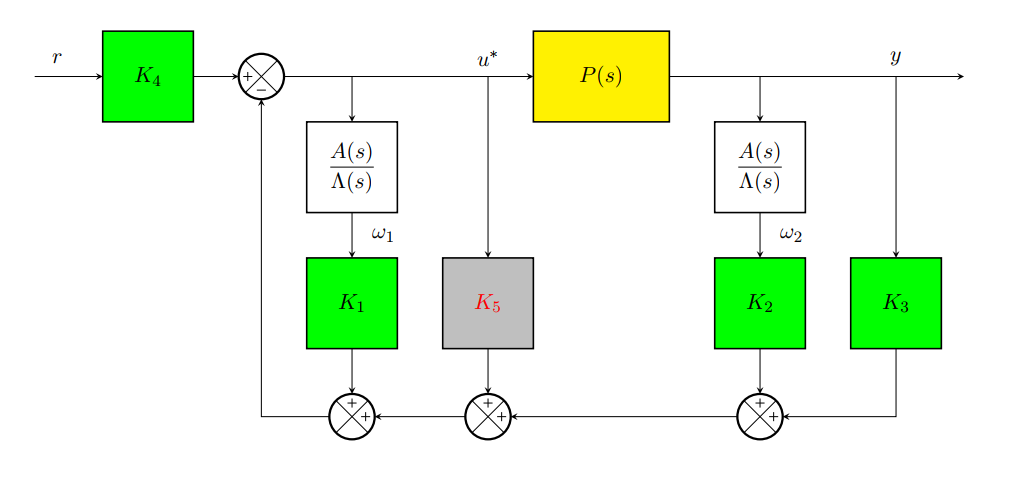
\includegraphics[width=15cm]{figs/mrac.png}
  \caption{Estrutura MIMO MRAC.}
  \label{mrac} 
\end{figure}

Utilizando o algoritmo de Monopoli, temos:
\begin{align}\label{eq:monopoli}
e &= \left[M(s)S\right]DL(s)L^{-1}(s)\left[u-\Omega^\intercal\Theta^*\right] \\
&=
\left[M(s)L(s)S\right]D\left[L^{-1}(s)u-L^{-1}(s)\Omega^\intercal\Theta^*\right]
\\
u &= L(s)\chi
\end{align}

Escolhmos:
\begin{align}
\chi &= \zeta^\intercal\Omega \\
u &= \Omega^\intercal\Omega +
\zeta^\intercal\dot{\Omega}
\end{align}

Como no caso $n^*=1$, � poss�vel provar que para todo modelo de refer�ncia
$M(s)$ existe $D_+$ tal que $M(s)L(s)S = M(s)L(s)L_1D_+L_1^\intercal$ � SPR.
Escolhendo a fun��o de Lyapunov:
\begin{align}
2V &= z^\intercal P_Mz+\tilde{\Theta}^\intercal|D|\Gamma^{-1}\tilde{\Theta}
\end{align}

podemos chegar na lei de adapta��o:

\begin{equation}
\dot{\Theta}(t) = -\text{sign}[D] \, \Gamma \, \zeta \, e(t),
\end{equation}

onde  $D = \text{diag}\left\{ d_1I_1, d)2I_2, \ldots , d_mI_m\right\}$

o erro converge assintoticamente para zero, em que $\Gamma =
\Gamma^\intercal > 0$ � uma matriz de ganhos positiva definida.

Observe que ainda falta analisar a estabilidade de $L(s)$. Nas notas de aula,
pode-se verificar a prova completa com a segunda lei de Lyapunov:
\begin{align}
V_L(z,\epsilon,\tilde{\Theta}) = V +\alpha\epsilon^\intercal P_1\epsilon
\end{align}

Neste trabalho, ser�o consideradas plantas de primeira e segunda ordens com grau
relativo 2 ($n^*=2$). Iremos simular e discutir o comportamento do erro e das
sa�das para varia��es das condi��es iniciais dos par�metros estimados
($\theta(0)$) e da planta ($y(0)$), do ganho de adapta��o $\Gamma$ e para
diferentes par�metros da planta e modelo.

\section{Implementa��o}

Foram considerados dois casos: caso em que $K_p$ � desconehcido; e caso em que
todos os par�metros da planta s�o desconhecidos.

\subsection{Caso em que apenas $K_p$ � desconhecido}

Consideremos a planta descrita pela eq.~\ref{eq:P}. A equa��o ideal para o
controlador 2DOF poode ser computada pela equa��o do erro eq.~\ref{eq:erro}:

\begin{align*}
u^* &=  \theta_1^{*\intercal}\omega_1 + \theta_2^{*\intercal}\omega_2 +
\theta_3y + \theta_4r \\
\omega_1 &= \frac{u^*}{\Lambda} \\
\omega_2 &=  \frac{y}{\Lambda} \\
\left(I - \theta_1^{*\intercal}\Lambda^{-1}\right)u^* &=
\theta_2^{*\intercal}\Lambda^{-1}y + \theta_3 y + \theta_4 r 
\end{align*}

Temos que: 

\begin{align*}
\frac{1}{\Lambda(s)} &= \begin{bmatrix}
\frac{1}{(s+\lambda_f)} & 0\\
0 & \frac{1}{(s+\lambda_f)}
\end{bmatrix}
\end{align*}

e

\begin{align*}
M(s) &= \begin{bmatrix}
\frac{\lambda^2}{(s+\lambda)^2} & 0\\
0 & \frac{\lambda^2}{(s+\lambda)^2}
\end{bmatrix}
\end{align*}

Voltando � equa��o da planta:

\begin{align*}
y &= PK_pu \\
\left(I - \theta_1^{*\intercal}\Lambda^{-1}\right)y &= \left(I -
\theta_1^{*\intercal}\Lambda^{-1}\right)P\bar{u}\\
\end{align*}

Como $P(s)$ � diagonal, temos $AP = PA$ (comuta). E $y = y_m$, logo:

\begin{align*}
\left(I - \theta_1^{*\intercal}\Lambda^{-1}\right)y_m &= P\left(I -
\theta_1^{*\intercal}\Lambda^{-1}\right)\bar{u}\\
\left(I - \theta_1^{*\intercal}\Lambda^{-1}\right)M(s)r &= P(\theta_2^{*\intercal}\Lambda^{-1}y_m +
\theta_3 y_m + \theta_4 r)\\
\left(I - \theta_1^{*\intercal}\Lambda^{-1}\right)M(s)r &= P(\theta_2^{*\intercal}\Lambda^{-1}M(s)r
+ \theta_3 M(s)r + \theta_4 r)\\
\left(I - \theta_1^{*\intercal}\Lambda^{-1}\right)M(s)r &= P(\theta_2^{*\intercal}\Lambda^{-1}M(s)
+ \theta_3 M(s) + \theta_4)r\\
\left(I - \theta_1^{*\intercal}\Lambda^{-1}\right)M(s) &= P(\theta_2^{*\intercal}\Lambda^{-1}M(s)
+ \theta_3 M(s) + \theta_4)\\
\end{align*}

\begin{align*}
\left(\begin{bmatrix}
1 & 0\\ 0 & 1
\end{bmatrix}-\theta_1^{*\intercal}\begin{bmatrix}
\frac{1}{(s+\lambda_f)} & 0\\ 0 & \frac{1}{(s+\lambda_f)}
\end{bmatrix}\right)\begin{bmatrix}
\frac{\lambda^2}{(s+\lambda)^2} & 0\\
0 & \frac{\lambda^2}{(s+\lambda)^2}
\end{bmatrix} &= \\
\begin{bmatrix}
\frac{1}{s^2} & 0\\0 & \frac{1}{s^2}
\end{bmatrix} \left(\theta_2^{*\intercal}\begin{bmatrix}
\frac{1}{(s+\lambda_f)} & 0\\ 0 & \frac{1}{(s+\lambda_f)}
\end{bmatrix}\begin{bmatrix}
\frac{\lambda^2}{(s+\lambda)^2} & 0\\
0 & \frac{\lambda^2}{(s+\lambda)^2}
\end{bmatrix} + \theta_3\begin{bmatrix}
\frac{\lambda^2}{(s+\lambda)^2} & 0\\
0 & \frac{\lambda^2}{(s+\lambda)^2}
\end{bmatrix} + \theta_4\right) & 
\end{align*}

Como todas as matrizes s�o diagonais, vamos resolver para o primeiro termo:

\begin{align*}
\left(1-\frac{\theta_1}{(s+\lambda_f)}\right)\frac{\lambda^2}{(s+\lambda)^2} &=
\frac{1}{s^2}\left(\frac{\theta_2}{(s+\lambda_f)}\frac{\lambda^2}{(s+\lambda)^2}
+ \theta_3 \frac{\lambda^2}{(s+\lambda)^2} + \theta_4\right)
\end{align*}

\begin{align*}
(\lambda^2-\theta_4)s^3 +
(\lambda^2\lambda_f - \theta_1\lambda^2 - \theta_4(\lambda_f + 2\lambda))s^2 +
(-\theta_3\lambda^2 - \theta_4(2\lambda\lambda_f+\lambda^2))s +
(-\theta_2\lambda^2 - \theta_3\lambda^2\lambda_f - \theta_4\lambda^2\lambda_f)
&= 0
\end{align*}

Resolvendo para $\theta$, temos:

\begin{align*}
\theta_4 &= \lambda^2\\
\theta_1 &= -2\lambda \\ 
\theta_3 &= -(2\lambda\lambda_f + \lambda^2) \\
\theta_2 &= 2\lambda\lambda_f^2\\
\end{align*}
 
Desssa forma, a lei de controle � descrita como:

\begin{align}
u^* = K_p^{-1}\left[2\lambda\lambda_f^2\Lambda^{-1}y -
(\lambda^2+2\lambda\lambda_f)y + \lambda^2r\right] - 2\lambda\Lambda^{-1} u
\end{align}

Utilizando o algoritmo de Monopoli~\ref{eq:monopoli}, temos:

\begin{align}
u &= \Omega^\intercal\Theta + \zeta^\intercal\dot{\Theta} - 2\lambda\omega_1\\
\nonumber \Omega_1^\intercal &= \left[\omega^\intercal \quad
u_2+2\lambda\omega_{1_2}\right] \\
\Omega_2^\intercal &= \left[\omega^\intercal\right] \\
\omega &= 2\lambda\lambda_f^2\omega_2 -
(\lambda^2+2\lambda\lambda_f)y + \lambda^2r \\
\omega_f &= L^{-1}(s)\omega \\
\nonumber \zeta_1^\intercal &= \omega_f^{\intercal}\left[I \quad \Theta_2\right]
\\
\zeta_2^\intercal &= \omega_f^\intercal \\
\dot{\Theta} &= -\text{sign}(D)\Gamma\zeta e
\end{align}

A implementa��o segue abaixo:

\lstinputlisting[style=myMatlab]{../matlab/1/mrac.m} 

\subsection{Caso onde todos os par�metros s�o desconhecidos}
\lstinputlisting[style=myMatlab]{../matlab/2/mrac.m}
%---------------------------------------------------------------------
\section{Resultados das simula��es}

%Simula��o utilizando \HI{\texttt{Matlab/Simulink}}.

%\subsection{Gradiente Normalizado}

Nas simula��es, procuramos avaliar o comportamento do sistema para as seguintes condi��es:
%
\begin{enumerate*}[label=(\roman*)]
\item condi��es iniciais $\theta(0)$ e $y(0)$;
\item Par�metros da planta e do modelo;
\item ganho de adapta��o $\Gamma$.
\end{enumerate*}

Apresentaremos os resultados obtidos atrav�s de simula��es no ambiente
\HI{\texttt{Matlab/Simulink}} e os discutiremos na pr�xima se��o.

\subsection{Caso em que apenas $K_p$ � desconhecido}

\begin{align*}
P(s) &= \begin{bmatrix}
\frac{1}{s^2} & 0\\
0 & \frac{1}{s^2}
\end{bmatrix} K_p, \\
K_p &= \begin{bmatrix}
\text{cos}(\phi) & \text{sin}(\phi)\\
-h\text{sin}(\phi) & h\text{cos}(\phi)
\end{bmatrix}\\
M(s) &= \begin{bmatrix}
\frac{\lambda^2}{s+\lambda^2} & 0\\
0 & \frac{\lambda^2}{s+\lambda^2}
\end{bmatrix}\\
r_1 &= \textrm{sin}(0.635t) + \textrm{sin}(4.567t)\\
r_2 &= \textrm{sin}(0.1t) + \textrm{sin}(1.1t)
\end{align*}

\subsubsection{Simula��o \#1}

Inicialmente, verificamos o comportamento do sistema para varia��es no
\textbf{par�metro de adapta��o} $\Gamma$.

\bigskip

\begin{align*}
  \phi &= \frac{\pi}{3} \,, & h &= 1 \,,\\
  y(0) &= \textbf{0} \,, & \gamma &= \HI{10}
    \,, \textrm{e} \, \HI{50}
\end{align*}

\begin{figure}[H]
  \centering
  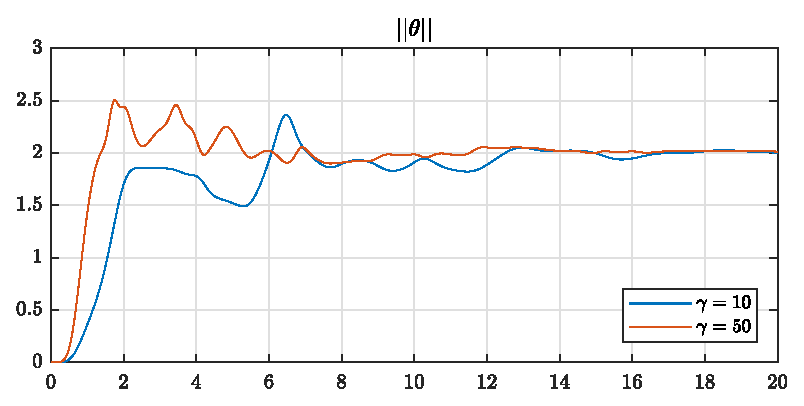
\includegraphics[width=12cm]{figs/1/modtheta/sim0gamma10gamma50.eps}
\end{figure}

\begin{figure}[H]
  \centering
  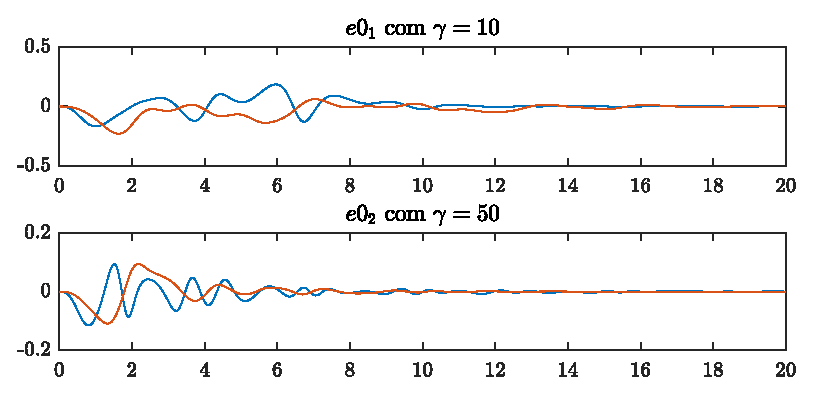
\includegraphics[width=12cm]{figs/1/e0/sim0gamma10gamma50.eps}
\end{figure}

%---------------------------------------------------------------------

\subsubsection{Simula��o \#2}

Verificamos agora o comportamento do sistema para varia��es na \textbf{condi��o inicial} $y(0)$.

\bigskip

\begin{align*}
  \phi &= \frac{\pi}{3} \,, & h &= 1 \,,\\
  y(0) &= \HI{$\textbf{0}$} \, e \, \HI{$\textbf{10}$} \,, & \gamma &= 10
\end{align*}

\begin{figure}[H]
  \centering
  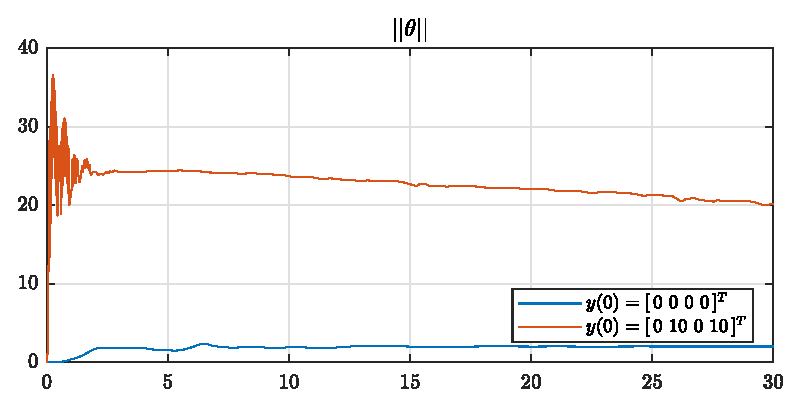
\includegraphics[width=12cm]{figs/1/modtheta/sim0y01y02.eps}
\end{figure}

\begin{figure}[H]
  \centering
  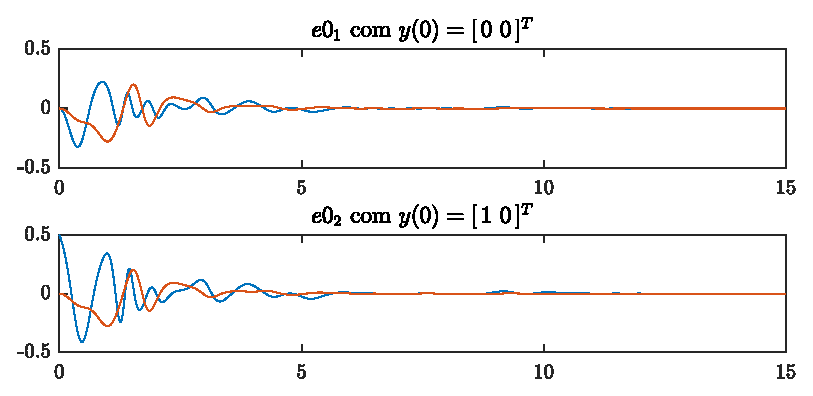
\includegraphics[width=12cm]{figs/1/e0/sim0y01y02.eps}
\end{figure}

% -----------------------------------------------------------------------------

\subsubsection{Simula��o \#3}

Verificamos o comportamento do sistema para varia��es na \textbf{fun��o de transfer�ncia da planta} $P(s)$.

\bigskip

\begin{align*}
  \phi &= \HI{$\frac{\pi}{3}$} \, e \, \HI{$\frac{\pi}{4}$} \,, & h &= \HI{1} \,
  e \, \HI{2} \,,\\
  y(0) &= \textbf{0} \,, & \gamma &= 10
\end{align*}

\begin{figure}[H]
  \centering
  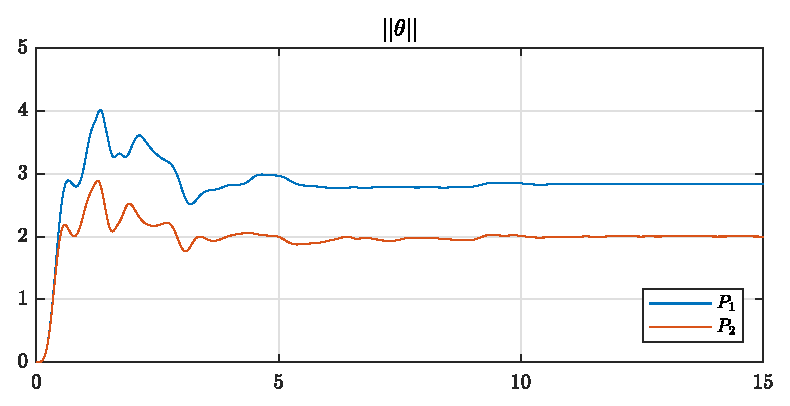
\includegraphics[width=12cm]{figs/1/modtheta/sim0P1P2.eps}
\end{figure}

\begin{figure}[H]
  \centering
  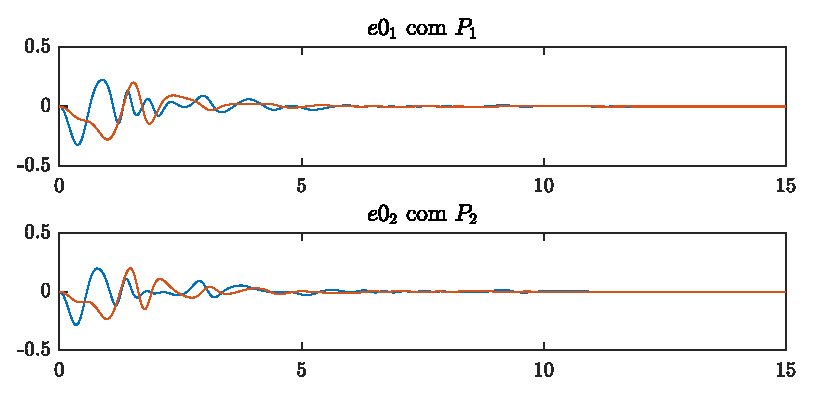
\includegraphics[width=12cm]{figs/1/e0/sim0P1P2.eps}
\end{figure}

% -----------------------------------------------------------------------------

\subsubsection{Simula��o \#4}

Verificamos o comportamento do sistema para varia��es na \textbf{fun��o de
transfer�ncia do modelo de refer�ncia} $P_m(s)$.

\bigskip

\begin{align*}
  \phi &= \frac{\pi}{3} \,, & h &= 1 \\
  y(0) &= \textbf{0} \,, & \gamma &= 10 \,, & \lambda &= \HI{1} \, e \, \HI{2} 
\end{align*}

\begin{figure}[H]
  \centering
  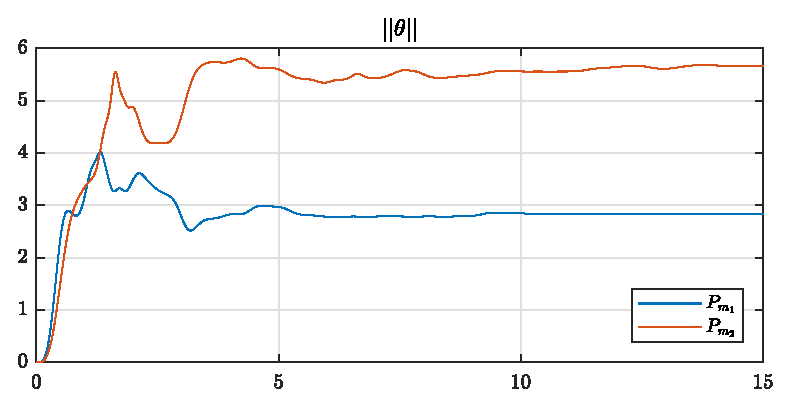
\includegraphics[width=12cm]{figs/1/modtheta/sim0Pm1Pm2.eps}
\end{figure}

\begin{figure}[H]
  \centering
  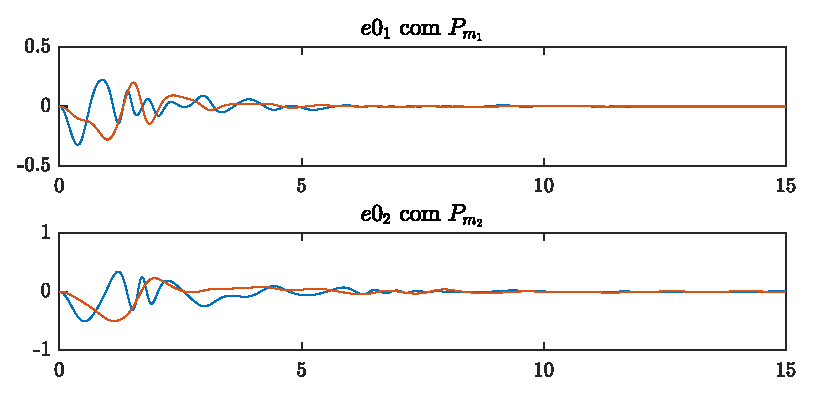
\includegraphics[width=12cm]{figs/1/e0/sim0Pm1Pm2.eps}
\end{figure}

\subsection{Caso em que todos os par�metros s�o desconhecidos}

\begin{align*}
P(s) &= \begin{bmatrix}
\frac{1}{s^2} & 0\\
0 & \frac{1}{s^2}
\end{bmatrix} K_p, \\
K_p &= \begin{bmatrix}
\text{cos}(\phi) & \text{sin}(\phi)\\
-h\text{sin}(\phi) & h\text{cos}(\phi)
\end{bmatrix}\\
M(s) &= \begin{bmatrix}
\frac{\lambda^2}{s+\lambda^2} & 0\\
0 & \frac{\lambda^2}{s+\lambda^2}
\end{bmatrix}\\
r_1 &= \textrm{sin}(0.635t) + \textrm{sin}(4.567t)\\
r_2 &= \textrm{sin}(0.1t) + \textrm{sin}(1.1t)
\end{align*}

\subsubsection{Simula��o \#1}

Inicialmente, verificamos o comportamento do sistema para varia��es no
\textbf{par�metro de adapta��o} $\Gamma$.

\bigskip

\begin{align*}
  \phi &= \frac{\pi}{4} \,, & h &= 1 \,,\\
  y(0) &= \textbf{0} \,, & \gamma &= \HI{100}
    \,, \textrm{e} \, \HI{20}
\end{align*}

\begin{figure}[H]
  \centering
  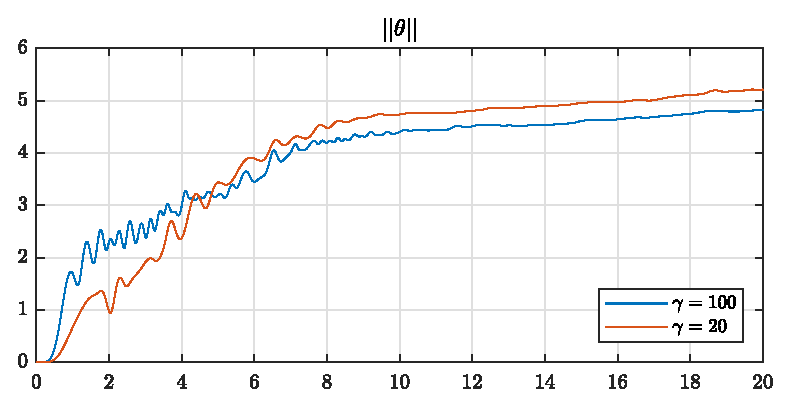
\includegraphics[width=12cm]{figs/2/modtheta/sim0gamma100gamma20.eps}
\end{figure}

\begin{figure}[H]
  \centering
  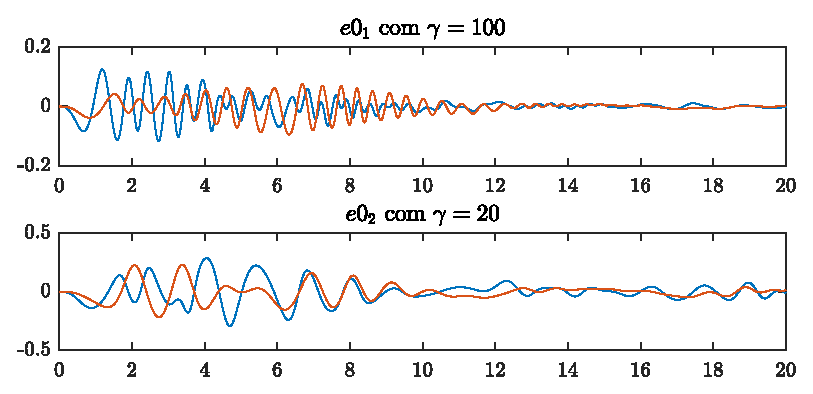
\includegraphics[width=12cm]{figs/2/e0/sim0gamma100gamma20.eps}
\end{figure}

%---------------------------------------------------------------------

\subsubsection{Simula��o \#2}

Verificamos agora o comportamento do sistema para varia��es na \textbf{condi��o inicial} $y(0)$.

\bigskip

\begin{align*}
  \phi &= \frac{\pi}{4} \,, & h &= 1 \,,\\
  y(0) &= \HI{$\textbf{0}$} \, e \, \HI{$\textbf{10}$} \,, & \gamma &= 100
\end{align*}

\begin{figure}[H]
  \centering
  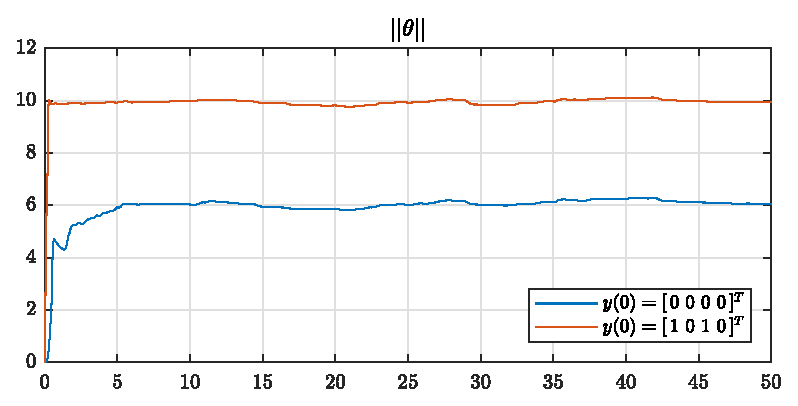
\includegraphics[width=12cm]{figs/2/modtheta/sim0y01y02.eps}
\end{figure}

\begin{figure}[H]
  \centering
  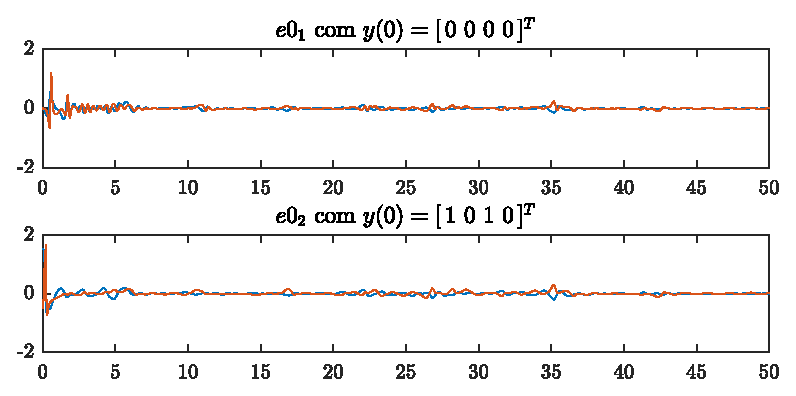
\includegraphics[width=12cm]{figs/2/e0/sim0y01y02.eps}
\end{figure}

% -----------------------------------------------------------------------------

\subsubsection{Simula��o \#3}

Verificamos o comportamento do sistema para varia��es na \textbf{fun��o de transfer�ncia da planta} $P(s)$.

\bigskip

\begin{align*}
  \phi &= \HI{$\frac{\pi}{4}$} \, e \, \HI{$\frac{\pi}{3}$} \,, & h &= \HI{1} \,
  e \, \HI{2} \,,\\
  y(0) &= \textbf{0} \,, & \gamma &= 100
\end{align*}

\begin{figure}[H]
  \centering
  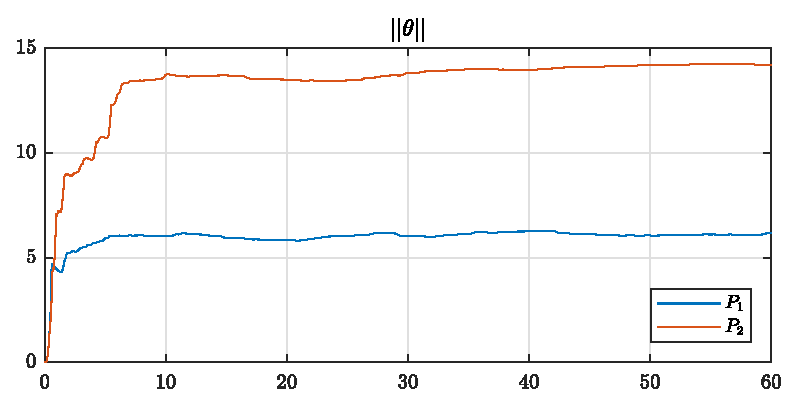
\includegraphics[width=12cm]{figs/2/modtheta/sim0P1P2.eps}
\end{figure}

\begin{figure}[H]
  \centering
  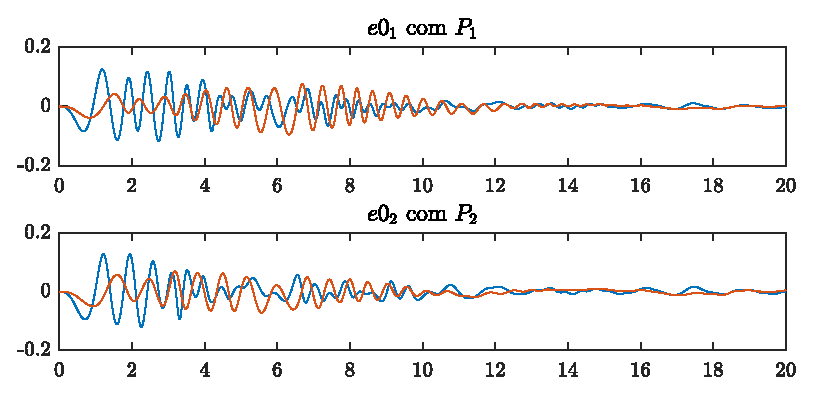
\includegraphics[width=12cm]{figs/2/e0/sim0P1P2.eps}
\end{figure}

% -----------------------------------------------------------------------------

\subsubsection{Simula��o \#4}

Verificamos o comportamento do sistema para varia��es na \textbf{fun��o de
transfer�ncia do modelo de refer�ncia} $P_m(s)$.

\bigskip

\begin{align*}
  \phi &= \frac{\pi}{4} \,, & h &= 1 \\
  y(0) &= \textbf{0} \,, & \gamma &= 100 \,, & \lambda &= \HI{1} \, e \, \HI{2} 
\end{align*}

\begin{figure}[H]
  \centering
  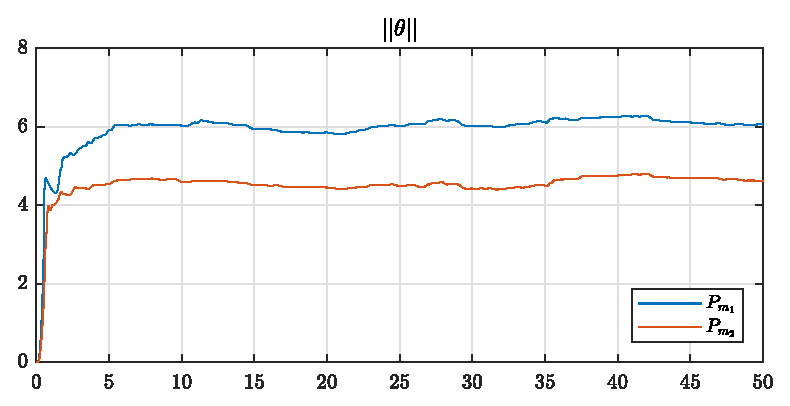
\includegraphics[width=12cm]{figs/2/modtheta/sim0Pm1Pm2.eps}
\end{figure}

\begin{figure}[H]
  \centering
  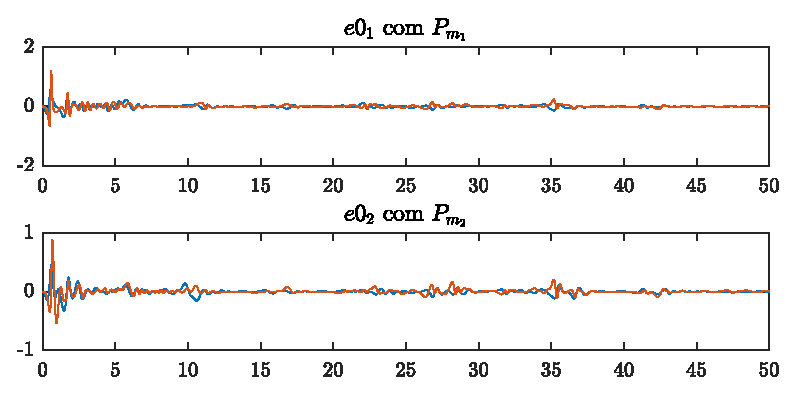
\includegraphics[width=12cm]{figs/2/e0/sim0Pm1Pm2.eps}
\end{figure}
 \newpage
%%---------------------------------------------------------------------
\section{Discuss�o}

Os resultados apresentados neste trabalho s�o semelhantes aos apresentados nos
trabalhos anteriores sobre MRAC, s� que aplicado a sistemas MIMO. Neste
trabalho, s�o abordados sistemas com duas entradas e duas sa�das e plantas de
segunda ordem com grau relativo 2. O filtro foi definido como mais simples
poss�vel.

Comparativamente, quando apenas $K_p$ � desconhecido (5 par�metros), o erro
converge rapidamente para zero, aproximadamente 15 segundos, usando ganhos de adapta��o
$\Gamma$ entre 10 e 50. O erro leva mais tempo para convergir para zero quando
todos os par�metros s�o desconhecidos (17 par�metros), aproximadamnte 30
segundos, o ganho de adapta��o deve ser bem maior (100), e o tempo de simula��o �, tamb�m, bem mais
elevado, pois a \textit{ode} calcula a derivada de 17 par�metros.

A \textbf{simula��o \#1} mostra o comportamento do sistema para varia��es no
ganho de adapta��o $\Gamma$. Como nos trabalhos anteriores, aumentar o ganho de
adapta��o garante converg�ncia mais r�pida, por�m mais oscila��es.

A \textbf{simula��o \#2} mostra o comportamento do sistema para varia��es nas
condi��es iniciais da planta $y(0)$. O sistema oscila mais para condi��es
iniciais da planta longe de zero. O transit�rio, por�m, foi menor para os
sistemas com condi��o inicial diferente de zero. Isso ocorre, pois os par�metros
entraram rapidamente em quadratura com o vetor de regressor.

A \textbf{simula��o \#3} mostra o comportamento do sistema para varia��es no
ganho de adapta��o na planta. A planta com maior deslocamento, $\phi =
\frac{\pi}{3}$, teve melhor transit�rio e convergiu mais r�pido,
mostrando que � dif�cil prever o comportamento comparativo quando
alteramos a planta.

A \textbf{simula��o \#4} mostra o comportamento do sistema para varia��es no
modelo. Modelos mais r�pidos apresentaram maiores oscila��es.
 
%---------------------------------------------------------------------
%\bibliographystyle{agsm}
%\bibliography{bib,coe736}

%---------------------------------------------------------------------
\end{document}
